% Cover letter: Product Designer (AI consumer-trends SaaS, remote), Spate
% CV: Sections/cv_product_designer_spate.tex -> cv_gen/cv_giovanni_tauro-spate.pdf
\documentclass[11pt,a4paper,sans]{moderncv}
% Shared preamble and header for the cover letters.
% One main file per application: cl_<company>.tex, built to
% cv_gen/coverletter_giovanni_tauro-<company>.pdf next to cv_giovanni_tauro-<company>.pdf.
% Paths (cl_gen/..., Pictures/...) are relative to the project root, as in the CV (see .latexmkrc).

\moderncvstyle{classic}
\moderncvcolor{blue}

\usepackage[scale=0.80]{geometry}
\setlength{\footskip}{136.00005pt}

\usepackage{fontawesome5}
% hyperref is loaded by moderncv itself; loading it here causes an option clash
\usepackage{xcolor}
\usepackage{graphicx}
\ifxetexorluatex
  \usepackage{fontspec}
  \usepackage{unicode-math}
  \defaultfontfeatures{Ligatures=TeX}
  \setmainfont{Latin Modern Roman}
  \setsansfont{Latin Modern Sans}
  \setmonofont{Latin Modern Mono}
  \setmathfont{Latin Modern Math}
\else
  \usepackage[T1]{fontenc}
  \usepackage{lmodern}
\fi

\usepackage[english]{babel}

% used for the PDF title and the letter closing; the visible header is \clheader below
\name{Giovanni}{Tauro}

% Header: #1 = headline under the name (same as the headline of the matching CV)
\newcommand{\clheader}[1]{%
\noindent
\begin{minipage}[c]{0.74\textwidth}
    {\Huge \textbf{Giovanni Tauro}}\\[-0.2em]
    {\small #1}\\[0.3em]

    \footnotesize
    \faMapMarker*~
    \href{https://www.google.com/maps/search/?api=1&query=Lecco+23900+Italy}
    {\color{blue}Bari-Lecco, Italy}
    \quad
    \faPhone*~
    \href{https://wa.me/393279437161}
    {\color{blue}+39 3279437161}
    \quad
    \faEnvelope~
    \href{mailto:giovanni.taurodi@gmail.com}
    {\color{blue}giovanni.taurodi@gmail.com}
    \\[-0.1em]

    \faLinkedin~
    \href{https://www.linkedin.com/in/giovanni-tauro-gt/}
    {\color{blue}LinkedIn}
    \quad
    \faGithub~
    \href{https://github.com/jotades}
    {\color{blue}GitHub}
    \quad
    \faGraduationCap~
    \href{https://scholar.google.com/citations?user=BS0aVGgAAAAJ&hl=it}
    {\color{blue}Scholar}
    \quad
    \faFilePdf~
    \href{https://www.notion.so/Giovanni-Tauro-2a7901d92f3a800b892af425c5875c6a}
    {\color{blue}Portfolio}
    \quad
    \faCubes~
    \href{https://grabcad.com/giovanni.tauro-3}
    {\color{blue}GrabCAD}

\end{minipage}
\hfill
\begin{minipage}[c]{0.18\textwidth}
    \raggedleft
    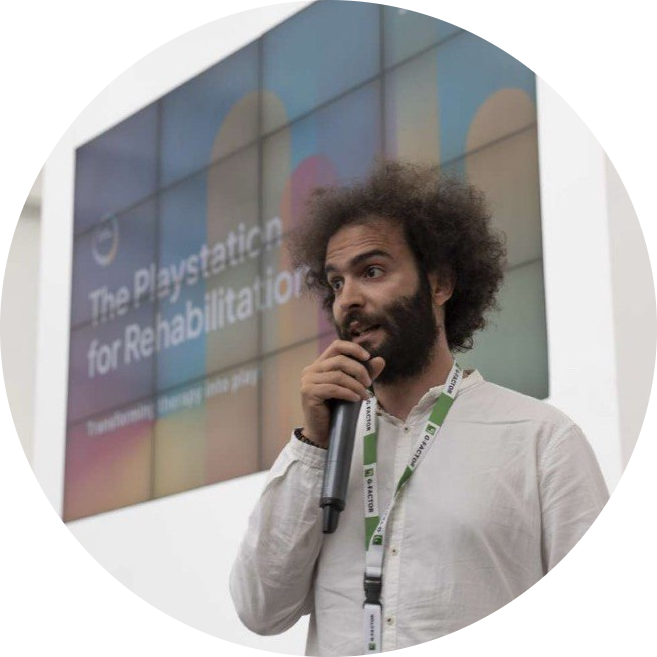
\includegraphics[width=2.8cm]{Pictures/Giovanni_pitch}
\end{minipage}
\vspace{0.1em}
}

\makeatletter
% the sender details are already in \clheader, so skip moderncv's own block
\@detailsfalse
% closing phrase, signature, name
\renewcommand*{\makeletterclosing}{%
  \@closing\\[0.6em]%
  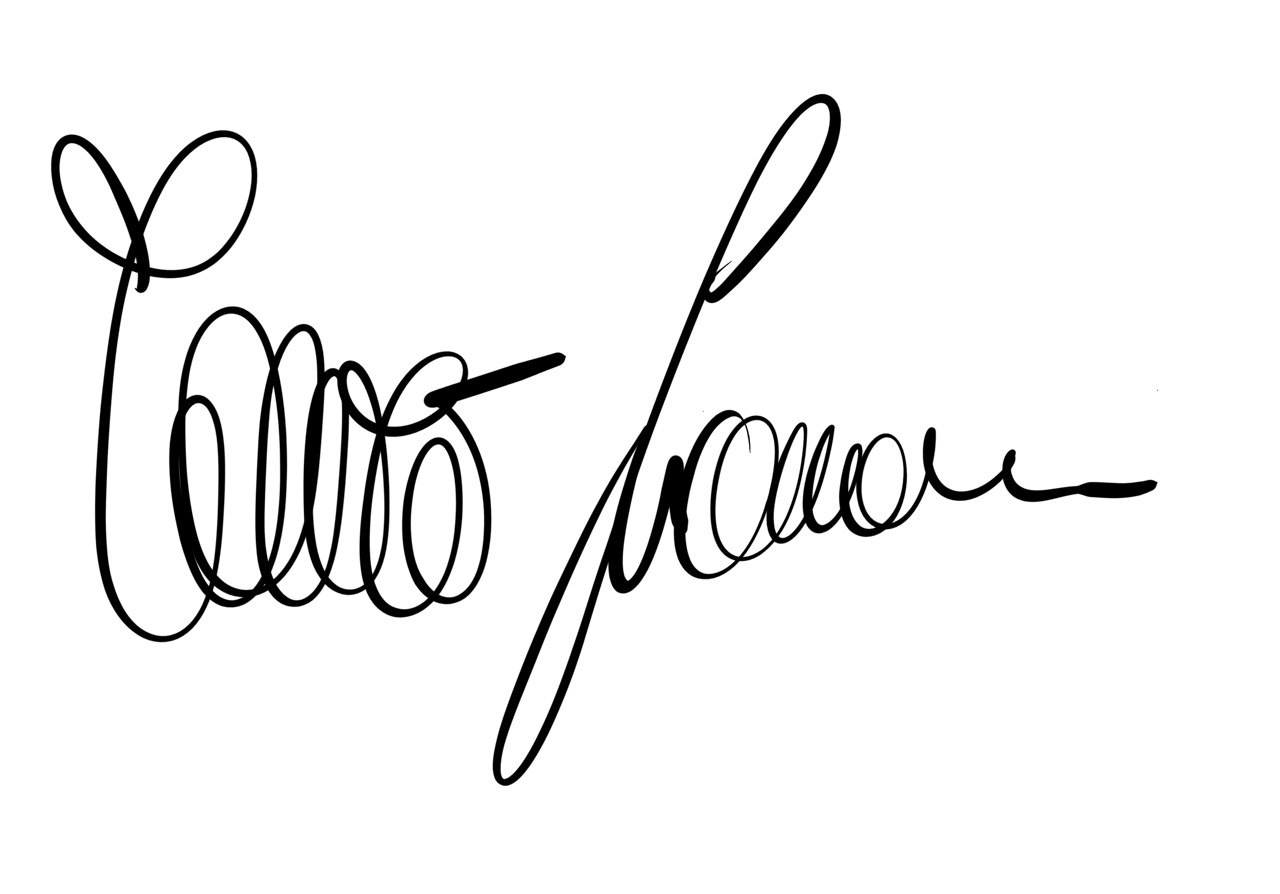
\includegraphics[height=1.2cm]{Pictures/sign_gt.jpg}\\[0.2em]%
  {\bfseries\@firstname~\@lastname}}
\makeatother


\begin{document}

\clheader{Product Designer | Data Tools, User Research \& AI Prototyping}

\recipient{Spate}{Remote}
\opening{Dear Spate Team,}
\closing{Sincerely,}
\makelettertitle

I am applying for the Product Designer role. I am Head of Product and co-founder of Rehabilia Technologies, and for more than five years I have designed tools for expert users at CNR-STIIMA, the Italian National Research Council. Most of my projects started without a spec, so bringing proposals instead of waiting for briefs is already how I work.

The clearest example is OmniTrack, my PhD project at the University of Bologna. It began as an open problem, indoor navigation for blind people, which I framed with users and researchers into an experience with audio and haptic feedback, tested with 16 blind participants. To make sense of the studies I designed OmniAnalytics, a dashboard for researchers with session browsing, time-series charts, trajectory playback and comparison tables. Much of the design work was in the exceptions: flows to fill a sensor gap, exclude a trial or relabel a session without ever altering the raw records, so every number on screen can be traced back to its source.

At Rehabilia I decide what we build and why. I run research with clinics and education centres on their pain points, the tools they use and how they decide what to buy, and turn it into written proposals, journey maps and priorities for engineering and clinical partners. Our device PhiCube reached a usability score of 85.8/100 (SUS) with 19 children. Papers, study protocols and proposals are a large part of my work, so I am used to writing decisions that have to stand on their own.

I use Claude and Claude Code every day, hold Anthropic's certifications for both, and use them to build quick prototypes that test an idea against real outputs. From the outside, the hard design problem in Spate's product seems to be trust: showing a forecast, how confident it is and what signals it rests on, so that a brand team can act on it. It is the same kind of problem I worked on in OmniAnalytics, and I would enjoy working on the LLM evaluations with your frontend lead. Consumer goods are not new to me either: my MSc thesis was the UX of an ultrasonic dental care device, and at Adidas I developed product concepts from trend and competitor research.

My products so far have served healthcare and research rather than B2B SaaS, and I have not yet built a design system that engineers adopted; these are the areas where I would expect to learn the most in my first months. Examples of my work are in the portfolio linked above.

I would welcome the chance to discuss the role further.

\makeletterclosing

\end{document}
